\documentclass{IEEEtran}
%\documentclass[peerreview,12pt,draftclsnofoot,journal,onecolumn]{IEEEtran}
%\documentclass[journal]{IEEEtran}

\IEEEoverridecommandlockouts
\usepackage{verbatim}
\usepackage{graphicx}
\usepackage{cite}
\usepackage{url}
\usepackage[cmex10]{amsmath}
\usepackage{amssymb}
\usepackage{amsmath}
\usepackage{algorithm,algorithmic}
%\usepackage{algpseudocode}
\usepackage{cases}
\usepackage[caption=false,font=footnotesize]{subfig}
\usepackage{color}
\usepackage{cite}
\usepackage{epstopdf}
\usepackage{calc}
\usepackage{array}
\usepackage{multirow}
\usepackage{hhline}

\DeclareMathOperator{\E}{\mathbb{E}}

\DeclareGraphicsExtensions{.pdf,.eps,.png,.jpg,.mps}
%\usepackage[nofiglist,notablist,nomarkers]{endfloat}
%\renewcommand{\efloatseparator}{\mbox{}}

%\renewcommand{\algorithmiccomment}[1]{\hfill $\triangleright$ #1}
\DeclareMathOperator{\cov}{cov}
\DeclareMathOperator{\diag}{diag}

\newtheorem{lemma}{Lemma}
\newtheorem{proposition}{Proposition}
\newtheorem{theorem}{Theorem}
\newtheorem{corollary}{Corollary}

\newcommand{\changed}[1] {{\color{blue}#1}}
\newcommand{\vc}[1]{\mathbf{c}_{#1}}
\newcommand{\vh}[1]{\mathbf{h}_{#1}}
\newcommand{\vp}[0]{\mathbf{p}}
\newcommand{\vb}[1]{\mathbf{b}_{#1}}
\newcommand{\vr}[1]{\mathbf{r}_{#1}}
\newcommand{\vu}[1]{\mathbf{u}_{#1}}
\newcommand{\vC}[1]{\mathbf{C}_{#1}}
\newcommand{\vone}[0]{\mathbf{1}}

%\renewcommand{\IEEEQED}{\IEEEQEDopen}

\begin{document}
\title{Agile Interferers Identification for Wideband Spectrum Sensing}
\author{TBD}
%\IEEEcompsocitemizethanks{\IEEEcompsocthanksitem Han Yan and Denijela Cabric are with the Department of Electrical Engineering, University of California, Los Angeles.}
%\IEEEauthorblockA{\\
%Email: yhaddint@ucla.edu, danijela@ee.ucla.edu}
%\thanks{The authors are with the Electrical Engineering Department, University of California, Los Angeles, CA, 90095, USA (email: \{pmurriza, rebeiz, danijela\}@ee.ucla.edu).}
%\thanks{Part of this work has been accepted to the proceedings of the Global Communications Conference (GLOBECOM), Dec. 3--7, 2012, Anaheim, CA, USA %\cite{Urriza2012}. Available: http://arxiv.org/abs/1210.8176.}
%\thanks{This work has been supported by the National Science Foundation under award number 1343389.}
\maketitle


%%%%%%%%%%%%%%%%%%%%%%%%%%%%%%%%%%%%%%%%%%%%%%%%%%%%%%%%%%%%%%%%%%%%%%%%%%%%%%%
%%%%%%%%%%%%%%%%%%%%%%%%%%%%%%%%%%%%%%%%%%%%%%%%%%%%%%%%%%%%%%%%%%%%%%%%%%%%%%%

\begin{abstract}
In a cognitive radio receiver, interferers degrade the performance of spectrum sensing due to various reasons. By identifying and removing the strong interferers in the wideband spectrum, the performance of spectrum sensing can be improved. We propose a novel cognitive radio receiver architecture and corresponding algorithm to efficiently identify strong interferers so that appropriate RF filtering can be applied. The proposed method features low ADC sampling rate as well as low computational complexity in the DSP. We provide the quantitative relationship between algorithm parameters and identification performance, which allows to reconfigure our system to reach required performance. The result is validated with Monte Carlo simulations. Compared with existing wideband signal detection method, namely swept-tuning periodogram estimation and compressive sensing, our proposed system offers a significant saving in terms of time and power consumption.
\end{abstract}

\IEEEpeerreviewmaketitle

% \begin{keywords}cognitive radio, spectrum sensing, compressive sensing
% \end{keywords}

%%%%%%%%%%%%%%%%%%%%%%%%%%%%%%%%%%%%%%%%%%%%%%%%%%%%%%%%%%%%%%%%%%%%%%%%%%%%%%%
%%%%%%%%%%%%%%%%%%%%%%%%%%%%%%%%%%%%%%%%%%%%%%%%%%%%%%%%%%%%%%%%%%%%%%%%%%%%%%%

\section{Introduction}
\label{sec:Introduction}
%Importance of CR
%With the fast development of wireless technology, it is expected that the number of mobile devices will exceed 20 billion by the year of 2025[ref need], with a factor of 10-100 more existing in the same physical area that share spectrum. However, most of the radio frequency (RF) band has already been assigned for different purposes. The seemingly scarcity of spectrum is due to the inefficiency of spectrum use[ref need]. Therefore, cognitive radio (CR) is a natural consequence. CR allows secondary user (SU) to utilize spectrum of licensed primary user (PU) in a non-interfering manner[ref need].

% spectrum sensing
\subsection{Motivations}
In the cognitive radios (CR) \cite{788210}, unlicensed secondary users opportunistically access the unoccupied spectrum bands for data transmission. CR transceivers need to reliably detect the unused bands. Spectrum sensing, as the enabling technology, has been extensively researched through theoretical analysis and simulations \cite{Hattab:2014bu,Axell:2012gs}. However, their hardware implementations still cannot provide desirable sensing performance. The early prototypes \cite{Yu:hm} met severe performance degradation when strong interferers are present. Reasons include gain saturation of amplifiers, inter-modulation interference and limited spurious free dynamic range of analog-to-digital converter (ADC) \cite{Razavi:2010jf}. 

% In Fig.~\ref{fig:multiband_interferers} the leakage of strong DTV interferer makes spectrum sensing unreliable for its neighbor primary user (PU). Interferers in GSM also cause detrimental effects. 

Conventional transceivers suppress interferers at radio frequency (RF) front-end by surface acoustic wave (SAW) bandpass filters. The lack of flexibility makes SAW filters not suitable for CR. Some recent works tend to actively suppress interferers or mitigate interference caused by them. Tunable notch filters are proposed to reject narrow band interferers in a programmable manner in \cite{Ghaffari:2013fn}. Works \cite{rebeiz2015spectrum,Zou:cj,Grimm:2014bt} reconstruct inter-modulation interference from interferers in order to compensate their impact. 

The receiver needs to detect dominant interferers in order to efficiently use the above techniques, because of the high implementation complexity of active suppressions. Therefore an interferers identification system is desired. The task is non-trivial because the interferers lie in a wideband and required resolutions varies for interferers in different bands, as shown in Fig.~\ref{fig:multiband_interferers}. Moreover, identification has a tight budget in terms of sensing time and energy consumption.


\begin{figure}
\begin{center}
\includegraphics[width=0.5\textwidth]{figure/wideband_interferers_multi_resolution}
\end{center}
\vspace{-6mm}
\caption{Illustration of multi-band interferers received by a typical spectrum sensing receiver.}
\vspace{-4mm}
\label{fig:multiband_interferers}
\end{figure}

% necessity of interferer identification and traditional way
\subsection{Related Works}
To the best of our knowledge, interferers identification among wide-band is not studied. We first briefly review existing methods applicable for this problem.

Conventional periodogram estimation method takes a snapshot of a certain frequency range in the spectrum. Detection of interferers is achieved by identifying striking frequency bins \cite{gardner1988statistical}. Swept-tuned spectrum analyzer (STSA) is usually adopted when interested signal is in a wide-band. Such system needs to scan synthesized frequency to down-convert signal components from different bands, and therefore it takes considerable sensing time \cite{6928507}. Moreover, it lacks flexibility for interferers' bandwidth. In order to retain enough resolution for narrow band interferers, increased numbers of FFT bins leads to high computationally complexity and energy consumption. 

% multi-band processing using compressive sensing
Compressive Sensing (CS) is a promising signal processing technique for sparse multi-band signal \cite{4472240}. In the recent years, several spectrum sensing system based on CS have been proposed, including random demodulation (RD), wideband modulation converter (WMC) and nonuniform sampling (NUS). However, CS is known to shift the front-end sampling burden to DSP end. Highly complex $l_1$ based optimization are required for a stable signal reconstruction. Till now most silicon implementations of CS based method were running off-line in CPU \cite{6502272,5678599}. A few studies report utilizes VLSI for real-time implementation \cite{6637036}. However, the high energy consumption makes such system unsuitable for a battery-powered cognitive radio transceivers.


% main contribution
\subsection{Contributions}
The main contributions are summaries as follows

\begin{itemize}
\item 
We propose a novel interferer identification architecture and corresponding algorithm. The receiver down-converts all interferers into baseband with controllable aliasing. Such analog processing is enabled by inserted pseudorandom calibration signal and a square-law device. This processing reduces burden of the local oscillator and ADC, resulting in a significant saving of energy consumption. The proposed algorithm reaches more than 90\% identification probability with the digitized signal. 

\item We present a theoretical analysis on identification probability. It serves as a guideline to design calibration signal and sensing time to reach identification performance.

\item We develop an energy consumption model for interferers identification system. This model enables a fair comparison between our system with the conventional STSA and CS-based wideband signal detection systems. We show the proposed system offers a significant saving in energy consumption without compromising identification performance or sensing time. 
\end{itemize}

% paper organization 
\subsection{Paper Outline}
The rest of the paper is organized as follows. Section II describes the signal model of interferers, the proposed system and algorithm. In section III we present a theoretical analysis on the statistical characteristics of power estimator. We analyze the identification algorithm and its performance in section IV. In section V, we present the numerical results and related discussions. The system level performance, including hardware resources, power and sensing time consumption, is analyzed in section VII together with a comparison with other wideband signal identification algorithms. We conclude the paper in Section VII.

% notation
\subsection{Notation}
Throughout this paper, we adopt the following notation. Vectors and matrices are presented by boldface lower case and upper case, respectively.  $(.)^T$denotes the vector or matrix transpose while $\mathbf{A}^{-1}$ is the inverse of a full rank matrix $\mathbf{A}$. $\Re (.)$ returns the real part of its argument. $\mathbb{P}(.)$ is the probability measure while $\E(.)$ is the expected value with respect to the underlying probability measure. $\{\mathbf{A}\}_{i,j}$ is component in $i^{th}$ row and $j^{th}$ column of matrix $\mathbf{A}$. $\mathrm{tr}(\mathbf{A})$ is evaluation of the trace of square matrix $\mathbf{A}$. $\mathrm{diag}(\mathbf{a})$ represents the diagonal matrix whose diagonal entries are determined by vector $\mathbf{a}$. Unit vector $\mathbf{e}_i$ is a vector with all components being 0 except the $i^{th}$ being 1. Matrix $\mathbf{I}$ and $\mathbf{J}$ are identity matrix and all one square matrix of appropriate dimensions, respectively. $\mathcal{N} \backslash \{i\}$ is a set operation to exclude element $i$ from set $\mathcal{K}$. $\jmath = \sqrt{-1}$ is the unit imaginary number.

%%%%%%%%%%%%%%%%%%%%%%%%%%%%%%%%%%%%%%%%%%%%%%%%%%%%%%%%%%%%%%
% 							Section 2: System Model
%
%%%%%%%%%%%%%%%%%%%%%%%%%%%%%%%%%%%%%%%%%%%%%%%%%%%%%%%%%%%%%

\section{System Model}
\label{sec:Model}
Consider a multi-band signal with $K$ components in lies in a wideband spectrum. Such signal $x(t)$ is expressed as
\begin{equation}
\label{eq:interferers_model}
x(t) = \sum\limits_{k=1}^{K} \sqrt{2P_{k}} \Re \left\{s_{k}(t) e ^{\jmath 2\pi f_{k}t+\phi_{k}}\right\} +w(t).
\end{equation}
In the above expression, $\sqrt{2P_{k}}$ is the amplitude of the signal in the $k^{th}$ band, and it is assumed to be constant during the identification procedure. $s_{k}(t)$ is its baseband signal with unit power, i.e., $\mathbb{E}\|s_k(t)\|^2=1$. The carrier frequency is $f_{k}$. $\phi_{k}$ is the unknown phase offset and $w(t)$ is the thermal noise. 

% Furthermore, we assume each baseband signal $s_{k}(t)$ has zero mean and its autocorrelation function $R_k(t,t+\tau)$ is periodic with $T_k$. The average autocorrelation function over its period is defined as 
% \begin{align}
% \bar{R}_k(\tau)\triangleq \frac{1}{T_k}\int_{0}^{T_k}R_k(t,t+\tau)dt.
% \end{align}

% We further assume all single carrier signals are linear modulated as
% \begin{align}
% s_{i} (t) = &\sum\limits_{k=-\infty}^{+\infty}I_{i,k}g_i(t-kT_i+\tau_i),
% %s_{im,i} (t) = &\sum\limits_{k=-\infty}^{\infty}I^{im}_{i,k}g_i(t+kT_i),
% \end{align}
% where $I_{i,k}$ is the $k^{th}$ complex symbols, $g_i(t)$ is the pulse shape function, $T_{i}$ is its symbol duration and $\tau_i$ is the timing offset. 
%Symbols are mutually independent and have unit power. The pulse shape function $g_i(t)$ has unit power as well, i.e., $\int_{-\infty}^{\infty}g_i^2(t)dt=T_i$.

We also assume we know the carrier frequency of each signal components, $f_{k}$. When a spectrum sensing system is capable to suppress $F (F \ll K)$ interferers, our goal is to identify the strongest $F$ signals among $K$ signals. 
 
We arrange the $K$ signals in descending order by their power and index them as $P_{n_1} \geq P_{n_2} \geq \cdots \geq P_{n_{K}}$. Hence the first $F$ index, $\{n_1,\cdots,n_{F}\}$, refers to dominant interferers. The correct identification is defined as the event $\mathcal{I} = \left\{\mathbb{T}=\{n_1,\cdots,n_{F}\}\right\}$, where $\mathbb{T}$ is the output of interferers identification module. We use the identification probability $\mathbb{P}(\mathcal{I})$ as a performance metric. 

%%%%%%%%%%%%%%%%%%%%%%%%%%%%%%%%%%%%%%%%%%%%%%%%%%%%%%%%%%%%
%
%                                   		    Subsection 2.2 Interferer Identification Blocker
%
%%%%%%%%%%%%%%%%%%%%%%%%%%%%%%%%%%%%%%%%%%%%%%%%%%%%%%%%%%%%

\section{Interferers identification system}
\label{sec:aigorithm}
The proposed interferers identification architecture is shown in Fig.~\ref{fig:system_schematic}. It consists of a pseudorandom calibration signal generator, a square-law device, low-pass filter, low-rate ADC and a DSP. We first describe our calibration signal, and then explain the analog signal processing happened in the front-end, followed by introducing the identification algorithm.

% calibration signals, which are basically multiple modulated spreading sequences, are inserted into suspecting bands where interferers lie in. The combined signal first passes through a square law device. It is then processed by a low-pass filter followed by an ADC with the sampling rate equal to the chip rate of the calibration signal. The digitized signal is further processed by a digital signal processor running proposed algorithm to provide power estimation of each of $K$ interferers of interest.

\begin{figure}
\begin{center}
\includegraphics[width=0.5\textwidth]{figure/system_all_TCCN}
\end{center}
\vspace{-6mm}
\caption{A spectrum sensing system capable to smartly steer reconfigurable notch filters for dominant interferers. Interferers identification module is detailed in the dashed box. Selected spectrum in its signal path are illustrated on the bottom of figure.}
\vspace{-4mm}
\label{fig:system_schematic}
\end{figure}


The multi-band calibration signals for $K$ candidate bands is the key to generate controlled aliasing. It is designed as
\begin{equation}
\tilde{c}(t) = \sqrt{2P_c}\sum\limits_{k=1}^{K} \Re \left\{c_k(t) e ^{\jmath 2\pi f_{k}t}\right\}.
\end{equation}
In the above expression, $\sqrt{2P_{c}}$ is the amplitude of each calibration signal, $P_c \gg \max{P_i}$. $c_{k}(t)$ is the power-normalized baseband calibration signal assigned for the $k^{th}$ band. It is linearly modulated from antipodal pseudorandom sequences $c_k[n]$, i.e.,
\begin{align}
c_k(t) = \sum\limits_{n=-\infty}^{+\infty}c_k[n]g\left(t-nT_c\right).
\end{align}
In this work, the symbol rate of the calibration signal is designed to be $1/T_c$. $g(t)$ refers to the unit-symbol-span rectangular pulse-shape function. 

% Note that  

% Practically, the spreading sequences $c_i[n]$ are antipodal pseudorandom codes, which can be generated by linear feedback shifted registers (LFSR) . But for simplicity in the following analysis, we assume such codes are independent and indentical distributed (i.i.d.) sequences with Rademacher distribution with probability mass function as
% \begin{align}
% f(c_i[n]) = 
% \begin{cases}
% 1/2, & \text{if } c_i[n]=1\\
% 1/2, & \text{if } c_i[n]=-1
% \end{cases}.
% \end{align}

We now explain the novel nonlinear processing used in our architecture. The output of square-law device (point \textcircled{3} in Fig.~\ref{fig:system_schematic}) is modeled as $y_{0}(t) = \beta_2(x(t)+\tilde{c}(t))^2$. Without loss of generality, we assume $\beta_2 =1/2$ since it can be easily scaled in the digital domain. In $y_0(t)$ there are signal components in both baseband and passband, as summarized in Appendix.~\ref{sec:components_in_y}. Analog anti-aliasing low-pass filter (LPF) with cutoff frequency $f_{\text{LPF}} = 2/T_c$ is then used to reject passband components. The remaining part is expressed as
\begin{align}
y (t)= & \sum\limits_{k=1}^{K}\sqrt{P_cP_{k}} \Re \left\{s_{k}(t)c^*_{k}(t)e^{\jmath \phi_{k}}\right\}\nonumber\\
&+\frac{1}{2}\sum\limits_{k=1}^{K}P_{k} |s_{k}(t)|^2+\frac{1}{2}\sum\limits_{k=1}^{K}P_{c} |c_{k}(t)|^2\nonumber\\
& +\sum\limits_{k=1}^{K}\sum_{l\in \mathcal{N}_k}\sqrt{P_cP_{k}} \Re \left\{s_{k}(t)c^*_{l}(t)e^{\jmath 2\pi (f_{k}-f_{l})t}e^{\jmath \phi_{k}}\right\}\nonumber\\
&+\sum\limits_{k=1}^{K}\sum_{l\in \mathcal{N}_k} \sqrt{P_{k}P_{l}} \Re \left\{s_{k}(t)s_{l}^*(t)e^{\jmath 2\pi (f_{k}-f_{l})t}e^{\jmath \left(\phi_{k}-\phi_{l}\right)}\right\}\nonumber\\
&+\sum\limits_{k=1}^{K}\sum_{l\in \mathcal{N}_k} P_c\Re\left\{c_{k}(t)c^*_{l}(t)e^{\jmath 2\pi\left(f_{k}-f_{l}\right)t}\right\}.
\label{eq:y_tilde_tilde}
\end{align}
where $\mathcal{N}_k\triangleq \{l:0<|f_k-f_l|<W_c/2\}$ is the set which contains index of bands whose distance to $k^{th}$ band is within $f_{\text{LPF}}$. Note that in (\ref{eq:y_tilde_tilde}) some approximation is made for analysis tractability. We kindly refer to Appendix.~\ref{sec:components_in_y} for the reasoning. Besides, since the interferers we are interested in are much higher than the noise floor, we omit terms depending on thermal noise $w(t)$ at the output of square-law device.


Signal $y(t)$ is then digitized by an ADC with sampling rate $f_s = 1/T_c$. The digitized signal is expressed as
\begin{align}
y [n]= & \sqrt{P_c}\sum\limits_{k=1}^{K}\sqrt{P_{k}} \Re \left\{s_{k}[n]c^*_{k}[n]e^{\jmath \phi_{k}}\right\}\nonumber\\
&+\frac{1}{2}\sum\limits_{k=1}^{K}P_{k} |s_{k}[n]|^2+\frac{K}{2}P_c\nonumber\\
&+\sqrt{P_c}\sum\limits_{k=1}^{K}\sum_{l\in \mathcal{N}_k}\sqrt{P_{k}}\Re \left\{s_{k}[n]c^*_{l}[n]e^{\jmath \omega_{k,l} n}e^{\jmath \phi_{k}}\right\}\nonumber\\
&+\sum\limits_{k=1}^{K}\sum_{l\in \mathcal{N}_k} \sqrt{P_{k}P_{l}} \Re \left\{s_{k}[n]s_{l}^*[n]e^{\jmath \omega_{k,l} n}e^{\jmath \left(\phi_{k}-\phi_{l}\right)}\right\}\nonumber\\
&+P_c\sum\limits_{k=1}^{K}\sum_{l\in \mathcal{N}_k} \Re \left\{c_{k}[n]c_{l}[n]e^{\jmath \omega_{k,l}n}\right\},
\label{eq:y_of_n}
\end{align}
where $\omega_{k,l} \triangleq 2\pi(f_k-f_l)/W_c$. We also use the fact that $c_l[n]$ is a real signal and $|c_k[n]|^2=1, \forall k$.



 \begin{algorithm}
 % \label{algorithm:esquential_estimation}
 \caption{Identification Algorithm}
 \begin{algorithmic}[1]
 \renewcommand{\algorithmicrequire}{\textbf{Input:}}
 \renewcommand{\algorithmicensure}{\textbf{Output:}}
 \REQUIRE Digitized sequences $y[n]$
 \ENSURE  Interferers index set $\mathbb{T}$
  \STATE{Compensate $y[n]$ by 
  \begin{align}
  \tilde{y}[n] = \sqrt{\frac{4}{P_c}}\bigg( &y[n] - \frac{K}{2}P_c- P_c\sum\limits_{k=1}^{K}\sum_{l\in \mathcal{N}_k} \Re \big\{e^{\jmath \omega_{k,l}n}\nonumber\\
  &\cdot c_{k}[n]c_{l}[n]\big\}\bigg).
  \label{eq:mitigate_cc_intermodulation}
  \end{align}
  }
  \FOR{$k = 1:K$}
  \STATE{Despreading with sequence $c_k[n]$
  \begin{align}
  y_{k}[n] = \tilde{y}[n]c_k[n]
  \label{eq:digital_correlator}
  \end{align}
  }
  \STATE{Low-pass filtering $y_k[n]$ by $h_k[n]$
  \begin{align}
  \hat{s}_{k}[n] = h_k[n] * y_{k}[n]
  \label{eq:digital_LPF}
  \end{align}
  }
  \STATE{Calculate power estimator
  \begin{equation}
  \hat{P}_{k} = \frac{1}{N}\sum\limits_{n=1}^{N}\|\hat{s}_{k}[n]\|^2.
  \label{eq:digital_power_estimator}
  \end{equation}
  }
  \ENDFOR
  % \STATE{Estimate effective noise floor via 
  % \begin{align}
  % \tilde{k} = \arg \min \hat{P}_k, \quad \hat{\sigma}_k^2 = \frac{\hat{P}_{\tilde{k}}T_{\tilde{k}}}{T_k} , \forall k
  % \label{eq:noise_est}
  % \end{align}
  % }
  % \STATE{Set the threshold for each interferer as 
  % \begin{align}
  % \gamma_k = Q_{\chi^2}(P_{\text{FA}})\hat{\sigma}_k^2, \forall k
  % \label{eq:threshold_gamma}
  % \end{align}
  % }
  \RETURN{Interferer index set $\mathbb{T} = \{k:\hat{P}_k>\gamma_k\}$}
 \end{algorithmic}
 \end{algorithm}


% \begin{align}
% \mathbf{\tilde{\tilde{y}}}= 2\sqrt{P_c}\sum\limits_{i=1}^{K} \sqrt{P_i}\mathbf{C}_i\mathbf{b}_i +\sum\limits_{i=1}^{K} P_i\mathbf{r}_i,
% \end{align}
% where
% \begin{align}
% \{\mathbf{b}_i\}_{k} \triangleq& s_{re,i}[k]+s_{im,i}[k], 1 \leq k\leq N,\\
% \{\mathbf{r}_i\}_{k} \triangleq& s_{re,i}^2[k]+s_{im,i}^2[k], 1 \leq k\leq N,\\
% \{\mathbf{c}_i\}_{k} \triangleq& c_{i}[k], 1 \leq k\leq N,\\
% \mathbf{C}_{i} \triangleq& \mathrm{diag}(\mathbf{c}_{i}),
% \end{align}
% Such signal is correlated with the corresponding spreading codes ($\mathbf{c}_{i}$) followed by averaging over the frame. The result from the $m^{th}$ frame is expressed as
% \begin{align}
% S_i[m] =&  \frac{1}{2\sqrt{P_c}N} \mathbf{\tilde{\tilde{y}}}^T\mathbf{c}_{i}.
% \label{eq: T_l}
% \end{align}
% where the factor ${1}/{2\sqrt{P_c}}$ is added in order to compensate scaling in the power estimation. It is worth noting that in (\ref{eq: T_l}) we imply a perfect timing between received signal and sequences used for the correlation, since such synchronization is inside the C2I2 system itself.

% After processing $M$ independent frames, the following estimator is used as power estimation of the $i^{th}$ interferer.
% \begin{align}
% \label{eq:estimator}
% \hat{P}_i =&  \frac{1}{M} \sum\limits_{m=1}^{M} S_i^2[m].
% \end{align}
The identification algorithm implemented in DSP is summarized in $\bf{Algorithm 1}$. We first compensate the self intermodulation terms from calibration signals, as expressed in (\ref{eq:self_inter_modulation}), since they are known. The power of each interferer is estimated via digital correlator (\ref{eq:digital_correlator}), LPF (\ref{eq:digital_LPF}), and power detector (\ref{eq:digital_power_estimator}). Note that in this architecture and associated algorithm, the chip rate of the calibration signals $T_c$ is a key parameter. In order to analyze the algorithm and design such parameters, we present a theoretical analysis quantitative relationship with the identification probability, as we are to show in the next section.

%%%%%%%%%%%%%%%%%%%%%%%%%%%%%%%%%%%%%%%%%%%%%%%%%%%%%%%%%%
%
% 									Section 3: Theoretical Analysis
%
%%%%%%%%%%%%%%%%%%%%%%%%%%%%%%%%%%%%%%%%%%%%%%%%%%%%%%%%%%

\section{Analysis of Identification Performance}
\label{sec:Theoretical}
In this section, we first analyze the interference components in the estimated interferers $\hat{s}_k[n]$. Then we present the statistic characteristics of the proposed power estimators $\hat{P}_k$ followed by the identification performance $\mathbb{P}(\mathcal{I})$.For analysis tractability, we assume all interferers have Gaussian signaling. Without loss of generality, we focus on the $k^{th}$ interferer.

\subsection{Interference analysis}
 After the signal $\tilde{y}[n]$ is despread by sequence $c_k[n]$ in (\ref{eq:digital_correlator}), the output is expressed as
 \newpage
\begin{align}
y_{k}[n] =\mathtt{s}^{(1)}_k[n]+\mathtt{s}^{(2)}_k[n]+ \mathtt{I}_k[n] +\mathtt{v}^{(1)}_k[n] +\mathtt{v}^{(2)}_k[n],
\label{eq:y_i_components}
\end{align}
where 
\begin{align}
\mathtt{s}^{(1)}_k[n] = &\sqrt{P_{k}}s_{k}[n]e^{\jmath\phi_{k}},\\
\mathtt{s}^{(2)}_k[n] = &\sqrt{P_{k}}s^*_{k}[n]c^2_k[n]e^{\jmath\phi_{k}}\nonumber\\
&+2\sqrt{P_{k}}\sum\limits_{l\in \mathcal{N}_k}\Re\left\{s_{k}[n]c_l[n]e^{\jmath\omega_{k,l}n}e^{\jmath\phi_{k}}\right\}c_k[n],\\
\mathtt{I}_k[n] = &\sum_{i\in \mathcal{N}_k}\sqrt{P_{i}}s_{i}[n]e^{\jmath\omega_{i,k}n}e^{\jmath\phi_{i}},\\
\mathtt{v}^{(1)}_k[n] = &\sum_{i\in \mathcal{N}_k}\sqrt{P_{i}}s^*_{i}[n]c^2_k[n]e^{\jmath\omega_{i,k}n}e^{\jmath\phi_{i}}\nonumber\\
&+2\sum\limits_{i=1,i\neq k}^{K}\sum\limits_{l\in \mathcal{N}_i\backslash\{k\}} \sqrt{P_{i}}\Re\left\{s_{i}[n]c_l[n]e^{\jmath\omega_{i,l}}e^{\jmath\phi_{i}}\right\}c_k[n]\nonumber\\
&+2\sum\limits_{i=1,i\neq k}^{K} \sqrt{P_{i}}\Re\left\{s_{i}[n]c_i[n]e^{\jmath\phi_{i}}\right\}c_k[n],\\
\mathtt{v}^{(2)}_k[n] = &2\sum\limits_{i=1}^{K}\sqrt{\frac{P_i^2}{P_c}}|s_i[n]|^2c_k[n] +2\sum\limits_{i=1}^{K}\sum\limits_{l\in \mathcal{N}_i} \sqrt{\frac{P_{i}P_l}{P_c}} \nonumber\\
&\cdot \Re\left\{ s_{i}[n]s^*_l[n] e^{\jmath\omega_{i,l}}e^{\jmath(\phi_{i}-\phi_{l})}\right\}c_k[n],
\end{align}
are the two catagories of signal and three categories of interference, respectively. Here $c_k[n]c^*_k[n] = 1, \forall k$ is used.
% \begin{align}
% \label{eq:S_l_expression}
% &y_{q}[n]  =  \underbrace{\sqrt{P_{q}}s_{q}\left(nT_s\right)e^{\jmath\phi_{q}}}_{\text{signal}}\nonumber\\
% &+\underbrace{\sum_{k\in \mathcal{N}_q\backslash\{q\}}\sqrt{P_{k}}s_{k}\left(nT_s\right)e^{\jmath\omega_{q,k}n}e^{\jmath\phi_{k}}}_{\text{non-spread interference}}\nonumber\\
% &+ \underbrace{\sum\limits_{k=1}^{K}\sum\limits_{l\in \mathcal{N}_k\backslash\{q\}} \sqrt{P_{k}}s_{k}\left(nT_s\right)c^*_l[n]c_q[n]e^{\jmath\omega_{k,l}}e^{\jmath\phi_{k}}}_{\text{spread interference 1}}\nonumber\\
% &+ \underbrace{\sum\limits_{k=1}^{K}\sum\limits_{l\in \mathcal{N}_k\backslash\{q\}} \sqrt{\frac{P_{k}P_l}{P_c}}s_{k}\left(nT_s\right)s^*_l(nT_s)c_q[n]e^{\jmath\omega_{k,l}}e^{\jmath(\phi_{k}-\phi_{l})}}_{\text{spread interference 2}}.
% \end{align}

The signal component, $\mathtt{s}_k^{(1)}[n]$, locates at the baseband and is not influenced by spreading sequence. The other signal component, $\mathtt{s}_k^{(2)}[n]$, have white spectrum due to the incorrelated spreading sequence attached with it. The non-spread interferences, $\mathtt{I}_k[n]$, come from interferers other than the $k^{th}$. They have nonzero frequency offset. The rest of components, $\mathtt{v}_k^{(1)}[n]$ and $\mathtt{v}_k^{(2)}[n]$, have white spectrum since they are spread by either two uncorrelated spreading sequences or one spreading sequence. Note that increasing the power of calibration signal $P_c$ reduces the power of $\mathtt{v}_k^{(2)}[n]$ while other components are not affected. It implies that we can improve SINR by using higher $P_c$. For that reason, we assume a sufficiently high $P_c$ is adopted and ignore $\mathtt{v}_k^{(2)}[n]$ in the following analysis.

For analysis sake, we assume the an ideal digital LPF $h_k[n]$, with no transition region and no delay, is applied to $y_k[n]$ in (\ref{eq:digital_LPF}). After filtering, the signal part $\mathtt{s}_k^{(1)}[n]$ remains. While $\mathtt{s}_k^{(2)}[n]$ has its spectrum reduced by a factor of $W_c/W_k$. The non-spread interferences $\mathtt{I}_i[n]$ are entirely rejected since they are outside the cutoff region of LPF $h_k[n]$, i.e., $\omega_{k,i} = 2\pi (f_k-f_i)/W_c>\pi W_k/W_c$. The interference $\mathtt{v}_k^{(1)}[n]$ has white spectrum, and thus the same factor of $W_c/W_k$ from $\mathtt{v}_k^{(2)}[n]$ is imposed to its power. 

Statistically, we treat the signal and the effective noise as $\mathtt{s}_k[n]$, $\mathtt{v}_k[n]$, respectively, as
\begin{align}
\hat{s}_{k}[n] = \mathtt{s}_k[n]+\mathtt{v}_k[n]
\label{eq:s_hat}
\end{align}
where both of them are modeled as Gaussian variables with zero mean and variance
\begin{align}
\sigma^2_{\mathtt{s}_k} = &\mathbb{E}\left\|\mathtt{s}^{(1)}_k[n]\right\|^2+\frac{W_k}{W_c}\mathbb{E}\left\|\mathtt{s}^{(2)}_k[n]\right\|^2\nonumber\\
= &P_{k}+\frac{3W_k}{W_c}P_k+\frac{2W_k}{W_c}\left|\mathcal{N}_k\right|P_k,
\label{eq:power_s}
\end{align}
\begin{align}
\sigma^2_{\mathtt{v}_k} = &\frac{W_k}{W_c}\mathbb{E}\left\|\mathtt{v}^{(1)}_k[n]\right\|^2\nonumber\\
=& \frac{W_k}{W_c}\sum\limits_{i\in\mathcal{N}_k}P_i\nonumber\\
&+\frac{2W_k}{W_c}\sum\limits_{i=1,i\neq k}^{K}\left(\left|\mathcal{N}_i\backslash\{k\}\right|+1\right)P_i.
\label{eq:power_n_int}
\end{align}
\onecolumn
\begin{align}
\text{SINR}_{k} 
% &\frac{\sigma^2_{\mathtt{s}_k}}{\sigma^2_{\mathtt{v}_k}} 
% = \frac{\text{var}\left(\mathtt{s}^{(1)}_k[n]\right)+\frac{W_k}{W_c}\text{var}\left(\mathtt{s}^{(2)}_k[n]\right)}{\frac{W_k}{W_c}\text{var}\left(\mathtt{v}^{(1)}_k[n]\right)} 
= \frac{P_{k}\left(1+\frac{3W_k}{W_c}+\frac{2W_k}{W_c}\left|\mathcal{N}_k\right|\right)}{\frac{W_k}{W_c}\sum\limits_{i\in \mathcal{N}_k}P_i+\frac{2W_k}{W_c}\sum\limits_{i=1,i\neq k}^{K}\left(\left|\mathcal{N}_i\backslash\{k\}\right|+1\right)P_i}.
\label{eq:power_n_int}
\end{align}

% We treat all of them as independent normally distributed 
% \begin{align}
% \mathtt{s} \sim &\mathcal{CN}\left(0,\sigma^2_{\mathtt{s}}\right),\nonumber\\
% \mathtt{n}_{\text{int}} \sim &\mathcal{CN}\left(0,\sigma^2_{\mathtt{n}_{\text{intra}}}\right),
% \end{align}
% Therefore the power estimator is normally distributed with
% \begin{equation}
% \mathbb{E}(\hat{P}_{q}) = \sigma^2_{\mathtt{s}}+\sigma^2_{\mathtt{n}_{\text{int}}},
% \end{equation}

% \begin{equation}
% \sigma^2(\hat{P}_{q}) = \frac{2}{N}\mathbb{E}^2(\hat{P}_{q}).
% \end{equation}

%%%%%%%%%%%%%%%%%%%%%%%%%%%%%%%%%%%%%%%%%%%%%%%%%%%%%%%%%%%%
%
% 											section 3.1
%
%%%%%%%%%%%%%%%%%%%%%%%%%%%%%%%%%%%%%%%%%%%%%%%%%%%%%%%%%%%%
\subsection{Accuracy of Power Estimator}
\label{sec:problem_formulation}
We first analyze the power estimator $\hat{P}_{q}$ in the following proposition

\begin{proposition}
\label{proposition:estimation_formulation}
Mean and variance of power estimator are
\begin{equation}
\mathbb{E}\left(\hat{P}_{q}\right) = P_{q}+\frac{2T_q}{T_c}\sum\limits_{k=1}^{K}\left|\mathcal{N}_k\backslash \{q\}\right|P_{k},
\label{eq:mean_of_estimator}
\end{equation}
\begin{equation}
\text{var}\left(\hat{P}_{q}\right) = \frac{1}{N'}\mathbb{E}^2\left(\hat{P}_{q}\right).
\label{eq:var_of_estimator}
\end{equation}
where $N'$ is the number of independent samples among $N$ samples. Approximately, $N' = NW_i/W_c$.
% where $\tilde{S}_{q,k}$ is defined as
% \begin{align}
% \tilde{S}_{q,k} = \frac{1}{\sqrt{N}}\sum\limits_{n=0}^{N-1}\sum\limits_{m=0}^{N-1}\bar{R}_k\left(\frac{|n-m|T_s}{N}\right)e^{\jmath \omega_{q,k}|n-m|}.
% \end{align}
\end{proposition}
\begin{IEEEproof}
Directly follows (\ref{eq:s_hat}), (\ref{eq:power_s}), and(\ref{eq:power_n_int}).
\end{IEEEproof}

The expression of estimator mean (\ref{eq:mean_of_estimator}) can be explained as follows. The first term represent the regular periodogram in $q^{th}$ band. The second term models the inter-band interference in power estimation. Such interference has same power among each sub-band.

Although our final goal is to identify dominant interferers and the impact from estimation precision is presented in the next subsection, there are several observations that we can make. Firstly, stronger interferers tend to be less affected by estimation offset than weaker interferers. Secondly, narrower bandwidth of interferers favors precise power estimation. An interesting scenario is all of interferers are single tones. As such the proposed method provide ideal power estimation performance. Thirdly, the impact of calibration signal chip rate plays a mixed role. Increasing the rate of $c(t)$ increasing the spreading. 
%%%%%%%%%%%%%%%%%%%%%%%%%%%%%%%%%%%%%%%%%%%%%%%%%%%%%%%%%%%%%
%
% 											section 3.2
%
%%%%%%%%%%%%%%%%%%%%%%%%%%%%%%%%%%%%%%%%%%%%%%%%%%%%%%%%%%
\subsection{Analysis of Identification Probability}
We fomulate the following hypothesis testing problem based on estimated signal $\hat{s}_q[n]$. In hypothesis $\mathcal{H}_0$, the interferer $i$ is absent, while in hypothesis $\mathcal{H}_1$, the interferer $i$ is present.
\begin{align}
\mathcal{H}_0: \hat{s}_i[n] = &\mathtt{v}_i[n],\nonumber\\
\mathcal{H}_1: \hat{s}_i[n] = &\mathtt{s}_i[n]+\mathtt{v}_i[n].
\end{align}

If the effective noise power is known, the optimal threshold with given false alarm constraint is
\begin{align}
\gamma_i =& Q^{-1}_{\chi^2_{N'}}\left(P_{FA}^0\right)\frac{\sigma^2_{\mathtt{v}_i}}{N'}\nonumber\\
\approx &\sigma^2_{\mathtt{v}_i}\left[1+\sqrt{\frac{2}{N'}}Q^{-1}\left(P_{FA}^0\right)\right].
\label{eq:threshold_calculation}
\end{align}
where $Q_{\chi^2_N}(.)$ is the right tail function of chi-square distrobution with degree of freedom $N$, $Q(.)$ is the right tail function of unit Gaussian distribution. $N'$ is the number of uncorrelated sample, since $\hat{s}_i[n]$ is white in the $2\pi W_i/W_c$ band. Approximately, $N' \approx NW_i/W_c$.

With the optimal threshold, the detection probability is expressed as
\begin{align}
P_D = Q\left(\frac{Q^{-1}\left(P_{FA}^0\right)-\sqrt{\frac{N'}{2}}\text{SINR}_i}{1+\text{SINR}_i}\right).
\end{align}

However, according to (\ref{eq:power_n_int}), the effective noise power $\sigma^2_{\mathtt{n}_i}$ is function of the power of interferers other than $i^{th}$, which are unknown. Therefore $\sigma^2_{\mathtt{n}_i}$ has to be estimated by the system in order to solve the hypothesis testing. Most likely, $K$ interferers are not all present, and the proposed effective noise power estimator $\hat{\sigma}_i^2$ in (\ref{eq:noise_est}) is the estimating power of an absent interferer, namely $P_{\tilde{k}} = 0$. Based on (\ref{eq:noise_est}) and (\ref{eq:mean_of_estimator}), the noise power estimator has its mean being
\begin{align}
\mathbb{E}(\hat{\sigma}_q^2) = \frac{T_{\tilde{k}}}{T_q}\mathbb{E}(\hat{P}_{\tilde{k}}) = \frac{2T_q}{T_c}\sum_{k=1}^{K}|\mathcal{N}_k\backslash\{\tilde{k}\}|P_k.
\end{align}
Although it has a slight offset with (\ref{eq:power_n_int}), such estimation is good enough for hypothesis testing as shown in the Section.~\ref{sec:Results}.

Using the estimated noise power, we can set the threshold based on an false alarm constraint (\ref{eq:threshold_gamma}). The detection probability is expressed as
\begin{align}
P_D = Q_{\chi^2}\left(\frac{\gamma}{\sigma^2_{\mathtt{s}}+\sigma^2_{\mathtt{n}}}\right).
\end{align}

The effective SNR, $\sigma_{\mathtt{s}}^2/\sigma_{\mathtt{n}}^2$, plays an key role in interferers identifying performance. Dominant interferers are easier to be identified due to high SNR. However, part of interferers can cause ditrimental effect on spetrum sensing, while they may not have good enough SNR. There are a couple of way to handle this problem. Increasing the collected samples is one way to improve SNR, but the increased identification duration may not be desirable. Increasing the calibration chip rate $1/T_c$ may not effectively reduce noise power since it potentially increase $\mathcal{N}_k$ as well. To further improve the identification performance, we propose a digital enhanced algortihm that actively estimate and mitigate cross-talk interference $\mathtt{n}[n]$ to increase SNR, as shown in Section.~\ref{sec:enhanced_algorithm}.
% In this subsection we analyze the identification probability. 

% The proposed method allows simultaneous periodogram estimation in multiple bands with the price of additional white inter-band interference and its power is usually high. We assume that intra-band interference is negligible compared with inter-band interference. Then we consider two special scenarios:
% \begin{itemize}
% \item the $(F+1)^{th}$ strongest interferer is much stronger than the inter-band interference
% \begin{equation}
% P_{n_{F+1}} \gg \frac{2}{N}\left(P_{tot} - P_{n_{F+1}}\right).
% \label{eq:F_plus_one_dominate}
% \end{equation}
% \item the $(F+1)^{th}$ strongest interferer is much weaker than the inter-band interference
% \begin{equation}
% P_{n_{F+1}} \ll \frac{2}{N}\left(P_{tot} - P_{n_{F+1}}\right).
% \label{eq:inter_dominate}
% \end{equation}
% \end{itemize}

% \begin{proposition}
% \label{proposition:2}
% When condition (\ref{eq:F_plus_one_dominate}) holds, an approximate expression of identification probability is
% \begin{align}
% \mathbb{P}(\mathcal{I}) \approx Q\left(\sqrt{\frac{M\left(P_{n_{F+1}}-P_{n_F}\right)^2}{P^2_{n_{F+1}}+P^2_{n_F}}}\right).
% \label{eq:ident_prob_f_plus_one}
% \end{align}
% \end{proposition}
% \begin{IEEEproof}
% See Appendix \ref{sec:proof_estimation_formulation_rc}.
% \end{IEEEproof}


% Under condition (\ref{eq:F_plus_one_dominate}), identification errors are mainly from failure of distinguish $(F+1)^{th}$ strongest interferer with the $F^{th}$. Therefore symbol rate ratio $N$ becomes irrelevant in such case because it only controls inter-band interference. High identification performance is expected when there are significant difference between $P_{n_{F+1}}$ and $P_{n_{F}}$. Required number of samples can easily be calculated from (\ref{eq:ident_prob_f_plus_one}) for targeted identification probability.


% \begin{proposition}
% \label{proposition:3}
% When condition (\ref{eq:inter_dominate}) holds, an approximate expression of identification probability is
% \begin{align}
% \mathbb{P}(\mathcal{I}) \approx Q\left(\sqrt{\frac{M\left(\mu_{t}-\mathbb{E}(\hat{P}_{n_F})\right)^2}{\sigma_t^2+\sigma^2(\hat{P}_{n_F})}}\right).
% \label{eq:ident_prob_interband}
% \end{align}
% where $\mu_{t}$ and $\sigma_t^2$ are the expectation and variance of normal order statistic, respectively. Their exact expressions are 
% \begin{align}
% \mu_{t} = &\frac{2P_{tot}}{N}\left(1+\frac{1}{\sqrt{M}}Q^{-1}\left(\frac{5}{8(K-F)+2}\right)\right)\\
% \sigma_{t}^2 = & \left(\frac{2P_{tot}}{N}\right)^2\frac{\pi^2}{12M\ln (K-F)}
% \end{align}
% \end{proposition}
% \begin{IEEEproof}
% See Appendix \ref{sec:proof_estimation_formulation_rc}.
% \end{IEEEproof}

% Under condition (\ref{eq:inter_dominate}), inter-band interference plays an overwhelming role in power estimation of signals and the weakest $K-F$ signals are deeply buried below such interference. The identification errors happens if the largest among those $K-F$ becomes higher than $\hat{P}_{n_F}$. Increasing $N$ can further reduce such interference effectively. However, we usually do not have much flexibility in choosing $N$ because condition \ref{eq:seperating_condition} has to be met. Increasing $N$ also put more burden in the ADC. 

% Identify signals below $2P_{tot}/N$ using proposed method is extremely difficult and may need undesirably huge number of samples. Fortunately in interferers identification application such scenario is very rare. 
%%%%%%%%%%%%%%%%%%%%%%%%%%%%%%%%%%%%%%%%%%%%%%%%%%%%%%%%%%%%%
%
% 											section 3.3
%
%%%%%%%%%%%%%%%%%%%%%%%%%%%%%%%%%%%%%%%%%%%%%%%%%%%%%%%%%%
\subsection{Comparison with other methods}
In this subsection, we briefly describe the STSA algorithm and its performance in the interferers identification application. 

STSA estimate periodogram of $K$ bands separately and compared the estimated power to identify dominant interferers. For fair comparison, we assume in sensing each band STSA uses the same frequency resolution as adopted in the proposed method. In other words, each $N/2$ complex samples are collected for the periodogram estimation of band $k$. Similar to the proposed method, time average is required to get reliable results. We mark such average number as $M_s$. 

Note that the power estimator of interferers are similar to (\ref{eq:mean_of_estimator}) and (\ref{eq:var_of_estimator}) except that there are not inter-band interference terms. When signals power meets condition (\ref{eq:F_plus_one_dominate}) the same number of average is required in both method. Since STSA need to collect samples for all $K$ bands, the total samples required in STSA is $K$ times greater than that in our proposed method.

In terms of CS, the existing theory cannot be directly applied to give analytical expression of identification performance. Therefore we rely on simulations for such comparison as shown in the Section \ref{sec:Results}.

%%%%%%%%%%%%%%%%%%%%%%%%%%%%%%%%%%%%%%%%%%%%%%%%%%%%%%%%%%
%
%								 Section VI: Digitally enhanced version
%
%%%%%%%%%%%%%%%%%%%%%%%%%%%%%%%%%%%%%%%%%%%%%%%%%%%%%%%%%%
\section{Implementation Issues}
In this section, we discuss practical issue of implementing the proposed interferere identification system.

\subsection{Thresholding via noise power estimation}
From (\ref{eq:threshold_calculation}), the optimal threshold $\gamma_i$ in detecting interferers requires the knowledge of effective noise power. From implementation perspective, $\sigma^2_{\mathtt{v}_i}$ needs to be estimated. 

From (\ref{eq:y_i_components}), if the PN sequence $c_i(t)$ is not inserted, components $\mathtt{s}^1_i[n]$ and $I_i[n]$ are no longer appearing. The measured power $\hat{P}_i$ is unbiased to 
\begin{align}
\mathcal{H}_0:& \mathbb{E}(\hat{P}^{\text{noise est}}_i) = \sigma^2_{\mathtt{v}_i}\nonumber\\
\mathcal{H}_1:& \mathbb{E}(\hat{P}_i) = \sigma^2_{\mathtt{v}_i}+\frac{W_i}{W_c}\left|\mathcal{N}_i\backslash \{i\}\right|P_i
\end{align}

Note that, when interferere $s_i(t)$ does not exist, the noise power estimation is unbiased. However, directly using (\ref{eq:threshold_calculation}) is not appropriate since noise measurement variance leads to extra false alarm. We take noise measurement variance into consideration and the false alarm contraint becomes
\begin{align}
\mathbb{P}\left(\sum \right) = P_{FA}^{0}
\end{align}

The threshold calculated by this procedure does not introduces additional false alarm rate. However, when interferere $s_i(t)$ exists, the biasing part causes certain compromise in the detection probab

In Algorithm 2, we summarized the procedure of determining threshold based on estimated noise power.
 \begin{algorithm}
 % \label{algorithm:esquential_estimation}
 \caption{Thresholdind based on Noise Power Estimation}
 \begin{algorithmic}[1]
 \renewcommand{\algorithmicrequire}{\textbf{Input:}}
 \renewcommand{\algorithmicensure}{\textbf{Output:}}
	\REQUIRE Digitized sequences $y[n]$
	\ENSURE  Interferers index set $\mathbb{T}$
	\STATE{Detect the strongest $D$ interferers via (\ref{eq:digital_power_estimator}) in Algorithm.1, with index $m_k, 1\leq k\leq D$.}
	\FOR{$k\leq D$}
	\STATE{Estimate crosstalk interference from $m_k^{th}$ interferer to others and compensate from $\tilde{y}[n]$
	\begin{align}
	\tilde{y}[n] = \tilde{y}[n] - \sum_{k\in \mathcal{N}_{m_k}}\hat{s}_{m_k}[n]c_{k}[n]e^{\jmath \omega_{m_k,k}n}.
	\label{eq:crosstalk_mitigation}
	\end{align}
	}
	\ENDFOR
	\STATE{Use post-mitigation signal $\tilde{y}[n]$ and Algorithm.1 for identification.}
	\RETURN{$\mathbb{T}$}
 \end{algorithmic}
 \end{algorithm}
 %%%%%%%%%%%%%%%%%%%%%%%%%%%%%%%%%%%%%%%%%%%%%%%%%%%%%%%%%%
%
%								 		Subsection: synchronizations
%
%%%%%%%%%%%%%%%%%%%%%%%%%%%%%%%%%%%%%%%%%%%%%%%%%%%%%%%%%%
\subsection{Synchronization}
In this sebsuction, we describe how synchronization is achieved in our system. Here synchronization represents the ssample level alignment in (\ref{eq:mitigate_cc_intermodulation}) and (\ref{eq:digital_correlator}). In the former step, time alignment between between digitized signal $y[n]$ and reconstructed self-intermodulation of calibration signals are important. Otherwise additional interference occurs. Equally important, (\ref{eq:digital_correlator}) requires sample level synchronization between $\tilde{y}[n]$ and PN sequence $c_i[n]$ in order to de-spread the interferer of interest. 

%%%%%%%%%%%%%%%%%%%%%%%%%%%%%%%%%%%%%%%%%%%%%%%%%%%%%%%%%%
%
%								 		Subsection: digital cross-talk mitigation
%
%%%%%%%%%%%%%%%%%%%%%%%%%%%%%%%%%%%%%%%%%%%%%%%%%%%%%%%%%%
\subsection{Digitally enhanced interferers identification}
\label{sec:enhanced_algorithm}
In order to improve the identification performance, we propose an enhanced identification algorithm.

In the original $\bf{Algorithm 1}$, we treat $\mathtt{n}_{\text{int}}[n]$ in $\hat{y}_q[n]$ as random interference. However, once a certain interferer is identified, its contribution to $\mathtt{n}_{\text{int}}[n]$ in estimating $\hat{y}_q[n]$ can be determined and compensated. Therefore a digitally enhanced version is to sequentially identify interferers and mitigate their cross-talk interference in identifying the sequel. We summarize the algorithm in $\bf{Algorithm 2}$.


% Once the strongest interferers $m_1$ is identified, it is not necessarily to treat $\mathtt{n}_{int}$ as the signal $\hat{s}_{m_1}[n]$ serves as a reference of $s_{m_1}(t)e^{\jmath \phi_{m_1}}$, which can be used to reconstruct part of the cross-talk interference in $\mathtt{n}_{\text{int}}[n]$. The cross-talk interference it introduces to identifying other interferers can be reconstructed as (\ref{eq:dominant_crosstalk}), 
% Note that the estimated interferer with highest power, $\hat{s}_{m_1}[n]$, has 

 \begin{algorithm}
 % \label{algorithm:esquential_estimation}
 \caption{Crosstalk Aware Identification Algorithm}
 \begin{algorithmic}[1]
 \renewcommand{\algorithmicrequire}{\textbf{Input:}}
 \renewcommand{\algorithmicensure}{\textbf{Output:}}
	\REQUIRE Digitized sequences $y[n]$
	\ENSURE  Interferers index set $\mathbb{T}$
	\STATE{Detect the strongest $D$ interferers via (\ref{eq:digital_power_estimator}) in Algorithm.1, with index $m_k, 1\leq k\leq D$.}
	\FOR{$k\leq D$}
	\STATE{Estimate crosstalk interference from $m_k^{th}$ interferer to others and compensate from $\tilde{y}[n]$
	\begin{align}
	\tilde{y}[n] = \tilde{y}[n] - \sum_{k\in \mathcal{N}_{m_k}}\hat{s}_{m_k}[n]c_{k}[n]e^{\jmath \omega_{m_k,k}n}.
	\label{eq:crosstalk_mitigation}
	\end{align}
	}
	\ENDFOR
	\STATE{Use post-mitigation signal $\tilde{y}[n]$ and Algorithm.1 for identification.}
	\RETURN{$\mathbb{T}$}
 \end{algorithmic}
 \end{algorithm}


We now present an analysis of the interference in $\hat{s}_q[n]$ after (\ref{eq:crosstalk_mitigation}). Let the $p^{th}$ interferer ($q\neq p$) be an identified one. After subtracting $\sum_{k\in\mathcal{N}_p}\hat{s}_p[n]c_k[n]e^{\jmath \omega_{m_k,k}n}$ from $\tilde{y}[n]$, the estimated $s_q[n]$ is expressed as 
\begin{align}
\hat{s}_{i}[n] = \mathtt{s}_i[n]+\tilde{\mathtt{n}}_i[n]
\end{align}
where
\begin{align}
&\tilde{\mathtt{n}}[n] = \sum\limits_{k=1,k \neq p,q}^{K}\sum\limits_{l\in \mathcal{N}_k\backslash\{q\}} \sqrt{P_{k}}s_{k}\left(nT_s\right)c^*_l[n]c_q[n]e^{\jmath\omega_{k,l}}e^{\jmath\phi_{k}}\nonumber\\
&+h_p[n]*\sum\limits_{k=1}^{K}\sum\limits_{l\in \mathcal{N}_k\backslash\{p\}} \sqrt{P_{k}}s_{k}\left(nT_s\right)c^*_l[n]c_p[n]e^{\jmath\omega_{k,l}}e^{\jmath\phi_{k}}.
\end{align}


Note that although interference from $s_p(t)$ is removed from the first terms, some additional interference from $\hat{s}_p[n]$ is introduced, as appear in the second term. When they are treated as i.i.d. distributed Gaussian variable. The variance of $\tilde{\mathtt{n}}_{\text{int}}$ is 
\begin{align}
\tilde{\sigma}^2_{\mathtt{n}} = &\frac{2T_q}{T_c}\left[\sum\limits_{k=1,k\neq p}^{K}\left|\mathcal{N}_k\backslash \{q\}\right|P_k+\frac{2T_p}{T_s}\sum\limits_{k=1}^{K}\left|\mathcal{N}_k\backslash \{p\}\right|P_k\right].
\end{align}
Compared with (\ref{eq:power_n_int}), the reduced interference power is
\begin{align}
\sigma^2_{\mathtt{n}}-\tilde{\sigma}^2_{\mathtt{n}} = \frac{2T_q}{T_c}\left[\left|\mathcal{N}_p\backslash \{q\}\right|P_p-\frac{2T_p}{T_s}\sum\limits_{k=1}^{K}\left|\mathcal{N}_k\backslash \{p\}\right|P_k\right].
\end{align}
The benefit of mitigating crosstalk interference from identified interferers is directly depends on $|\mathcal{N}_p|P_p$. Therefore the mitigation algorithm is carried out by $D$ times ($D<F$).

%%%%%%%%%%%%%%%%%%%%%%%%%%%%%%%%%%%%%%%%%%%%%%%%%%%%%%%%%%
%
%								 		Section VI: Simulation
%
%%%%%%%%%%%%%%%%%%%%%%%%%%%%%%%%%%%%%%%%%%%%%%%%%%%%%%%%%%
\section{Numerical Results and Discussion}
\label{sec:Results}
In this section, we use numerical method to verify analysis in the previous section. Except otherwise mentioning, the simulation parameters are from Table \ref{tab:table1}. For clarity, we set all interferers to have identical modulation type and pulse-shape function in all the simulations. 
%%%%%%%%%%%%%%%%%%%%%%%%%%%%%%%%%%%%%%%%%%%%%%%%%%%%%%%%
%
%											 section 4.1
%
%%%%%%%%%%%%%%%%%%%%%%%%%%%%%%%%%%%%%%%%%%%%%%%%%%%%%%%%
\subsection{Verification of Identification Performance Analysis}
In this part, we verified previous analysis of identification probability. We consider $K = 8$ bands and each band has $n_k = 16$ sub-bands. In the simulation, 3 interferers are randomly generated from $K = 128$ sub-bands and their power are randomly generated as well. The weakest one has power $P_{lr}$ and their total power is 0 dBm. 

\begin{table}
\caption{Simulation Parameters}
\centering
\begin{tabular}{|m{3.5cm}|c|}
\hline 
Parameters & Values\tabularnewline
\hline 
\hline 
Investigating Bands & $K = 8$\tabularnewline
\hline 
Sub-bands per Band & $n_k = 16$\tabularnewline
\hline 
Total band Number & $K = 128$\tabularnewline
\hline 
Interferers Modulation Type & 4-QAM \tabularnewline
\hline 
Interferers Bandwidth & $B_{k} = 200$ KHz\tabularnewline
\hline 
Interferers Pulse Shape  & Root raise cosine (RRC) $^{a}$\tabularnewline
\hline 
Period of PN sequences & $N$ = 32 \tabularnewline
\hline 
Power of calibration signal & $P_c = 10$ dBm \tabularnewline
\hline
% Calibration Signal Symbol Period &  $ T_{c} =2.5\times10^{-7}$ second\tabularnewline
% \hline 
Targeted Interferers & $ F = 3$\tabularnewline
\hline 
Monte Carlo Runs & $10,000$\tabularnewline
\hline
\multicolumn{2}{l}{$a:$ RRC has 0.5 roll-off factor and 11 symbol spans.}\\
\end{tabular}
\label{tab:table1}
\end{table}


\begin{figure}
\begin{center}
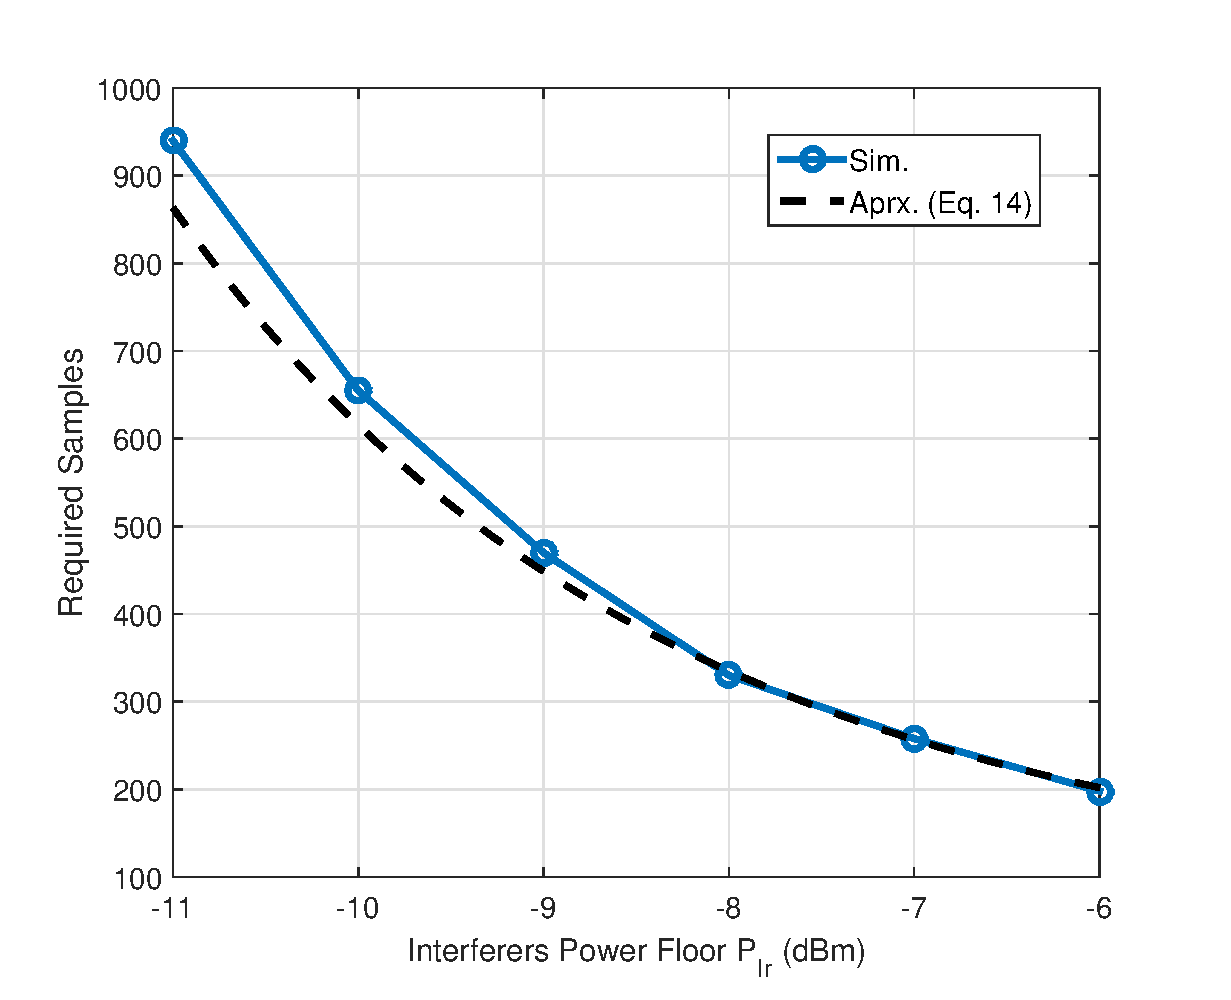
\includegraphics[width=0.5\textwidth]{figure/sim_vs_theo_allnew}
\end{center}
\caption{Required number of samples to get targeted identification performance with different options of calibration signal power.}
\label{fig:sim_vs_theo}
\end{figure}


The simulated value of required samples in reaching 90\% identification probability is plotted as solid curve in Fig.~\ref{fig:sim_vs_theo}. The required samples predicted by (\ref{eq:ident_prob_interband}) is plotted as dashed curve. Note that the total required samples is the product of frame number $M$ with samples per frame $N$. Non-integer value of $M$ from interpolation are allowed to generate a smooth curve. 

The result verifies our analysis since both curve are well matched. Besides, we observe that low sample number is required for large $P_{lr}$. In other words, our system benefits when interferers are similar in their power. Required sample increases for small power floor $P_{lr}$, because identification is more vulnerable to cross-talk interference in this situation.

%%%%%%%%%%%%%%%%%%%%%%%%%%%%%%%%%%%%%%%%%%%%%%%%%%%%%%%%
%
%											 section 4.2
%
%%%%%%%%%%%%%%%%%%%%%%%%%%%%%%%%%%%%%%%%%%%%%%%%%%%%%%%%
\subsection{Identification Performance under model mismatch}
For mathematical tractability, we overlooked some factors in the analysis. For example, calibration signal power can not be arbitrarily large, intra-band interference from power leakage may also introduce additional identification error.

In this part, we rely on simulation to study the performance under model mismatch. The following effects are mainly considered.
\begin{itemize}
\item Non-zero side-lobe in periodogram estimation, $\tilde{S}[k] \neq 0, \forall k\neq 0$.
\item Finite value of calibration signal power, $P_{i,k}/P_c \neq 0$
\end{itemize}

\begin{figure}
\begin{center}
\includegraphics[width=0.5\textwidth]{figure/different_Pc_dependent_frames}
\end{center}
\caption{xxx}
\label{fig:sim_vs_theo4}
\end{figure}

%%%%%%%%%%%%%%%%%%%%%%%%%%%%%%%%%%%%%%%%%%%%%%%%%%%%%%%%
%
%											 section 4.2
%
%%%%%%%%%%%%%%%%%%%%%%%%%%%%%%%%%%%%%%%%%%%%%%%%%%%%%%%%
\subsection{Comparison with STSA}
The simulation setting is same as in Table.~\ref{tab:table1} except the number of active blockers are assumed to be Poisson distributed with rate $\lambda=2$ and power of active blockers are uniformly distributed from -30 to 0 


\begin{figure}
\begin{center}
\includegraphics[width=0.5\textwidth]{figure/comparison_STSA_prob1}
\end{center}
\caption{Probability of identifying the $F$ strongest interferers with different number of samples. Note that STSA needs at least 256 samples to make identification while this works needs only 32.}
\label{fig:sim_vs_theo3}
\end{figure}

\begin{figure}
\begin{center}
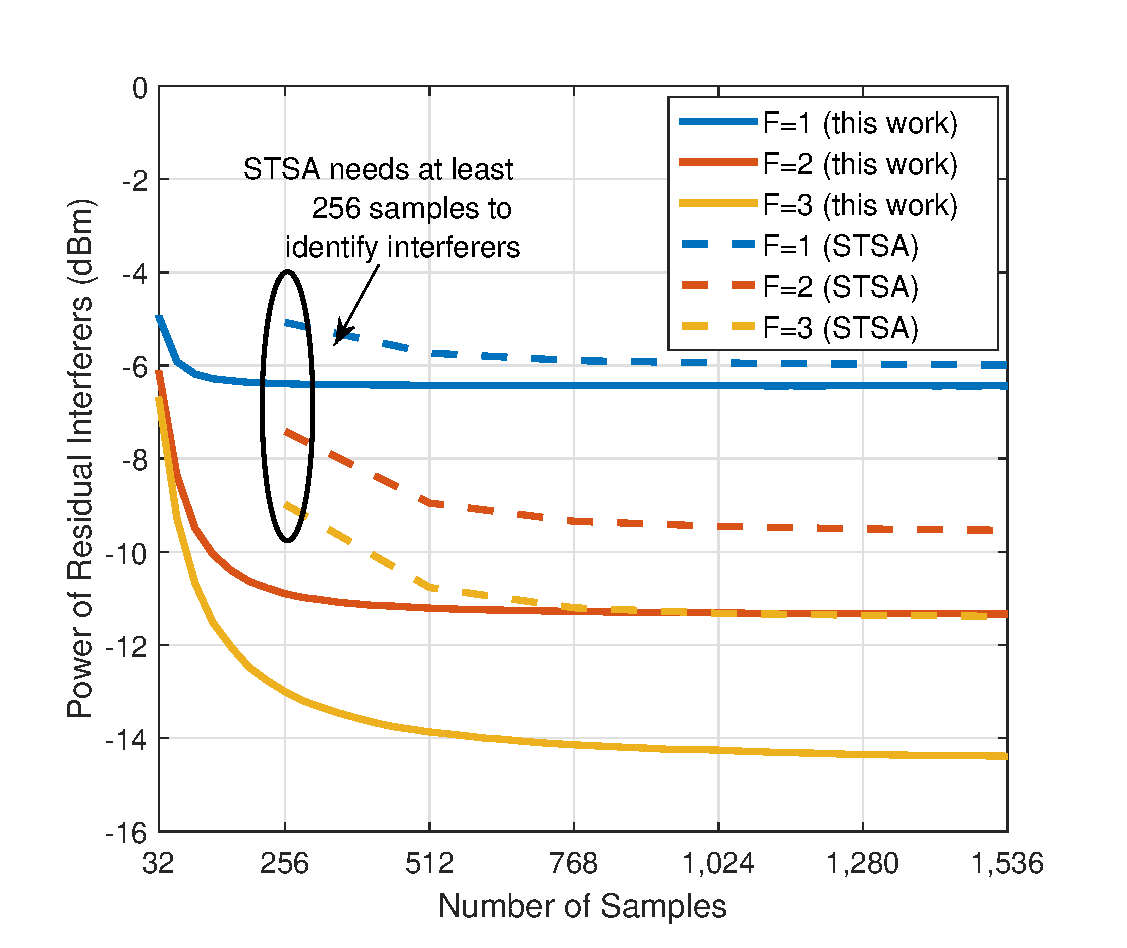
\includegraphics[width=0.5\textwidth]{figure/comparison_STSA_resd}
\end{center}
\caption{Average residual power of interferers after $F$ notch filters suppress identified interferers. Note that STSA needs at least 256 samples to make identification while this works needs only 32.}
\label{fig:sim_vs_theo2}
\end{figure}
%%%%%%%%%%%%%%%%%%%%%%%%%%%%%%%%%%%%%%%%%%%%%%%%%%%%%%%%%%%%%%%%%%%%%%%%%%%%%%%%%%%%%%
%
%											 section 4.3
%
%%%%%%%%%%%%%%%%%%%%%%%%%%%%%%%%%%%%%%%%%%%%%%%%%%%%%%%%%%%%%%%%%%%%%%%%%%%%%%%%%%%%%%
\subsection{Comparison with CS}
Compressive sensing is a promising technique to detect sparse signals in a wideband. However, it is known that the reconstructed signals often have a distortion in its carrier frequency. Therefore when fine frequency resolution is required, CS is not necessarily the best candidate. Besides, in most literature signals are modeled as multi-tones with same amplitude, its performance in detecting 

In this section, we consider applying CS in interferers identification. For fair comparison, we consider a wideband from 500MHz to 5GHz and a frequency resolution is still 200KHz as assumed in the previous section. In such 22500 bands we consider the number of interferers follows Poisson distribution with $\lambda = 2$. Such setting results in an extremely sparse signals with sparsity far less than $0.1\%$. The power of interferers are also uniformly distributed from -15 to 0 dBm. 

Front-end architecture of CS is chosen to be 

\begin{figure}
\begin{center}
\includegraphics[width=0.5\textwidth]{figure/cs_v2}
\end{center}
\caption{xxx}
\label{fig:sim_vs_theo1}
\end{figure}

%%%%%%%%%%%%%%%%%%%%%%%%%%%%%%%%%%%%%%%%%%%%%%%%%%%%%%%%%%%%%%%%%%%%%%%%%%%
%
%								 		Section : Hardware resource comparison
%
%%%%%%%%%%%%%%%%%%%%%%%%%%%%%%%%%%%%%%%%%%%%%%%%%%%%%%%%%%%%%%%%%%%%%%%%%%%
\section{System Performance Comparison}
In this section, we compare our system with the STSA and CS-based system. The comparison metrics are sensing/processing time and system level power consumption.
\subsection{RF front-end}
\begin{figure}
\begin{center}
\includegraphics[width=0.45\textwidth]{figure/STPE_system}
\includegraphics[width=0.45\textwidth]{figure/CS_system}
\end{center}
\vspace{-6mm}
\caption{The front-end architecture of (a) The STSA system, (b) the CS-MWC system}
\label{fig:other_systems}
\vspace{-4mm}
\end{figure}

A typical STSA system is presented in the upper part of Fig.\ref{fig:other_systems}. Each time an approximate sinusoid wave at frequency $f_{LO}$ is synthesized by PLL. The range of periodogram that can be estimated is $[f_{LO}-f_s/2,f_{LO}+f_s/2]$. The sensing time of each band depends on required frequency resolution. The entire interested band can be inspected by sweeping LO. Since it takes a certain amount of time before PLL settles at a new frequency, a switch time for PLL settling is expected between sensing consecutive bands.

It is worth noting that there is a time-complexity trade-off in the STSA system. Shorter sensing time can be achieved by using multiple parallel paths. For example, by building $q$ identical paths in the STSA system, a band of $q f_s$ can be digitized simultaneously as the cost of additional PLL, LPF and ADC. In order for a fair comparison, we adopt STSA system as shown in Fig.\ref{fig:other_systems}.

The sensing time can be roughly calculated by
\begin{align}
T_{STSA} = \frac{B_{tot}}{f_s}(\frac{1}{B_{res}}+T_{sw})
\end{align}
where $f_s$ is the sampling frequency, $1/B_{res}$ is the required observation time window for required frequency resolution $B_{res}$, $T_{sw}$ is the time for PLL switching to different frequencies.

The energy consumption of the STSA front-end is
\begin{align}
P_{STSA}= &P_{PLL}+P_{ADC}^{FOM}\cdot 2^{ENOB}\cdot f_s 
\end{align}
where $P_{ADC}^{FOM}$ represents for the figure of merit (FOM) of ADC. Scaling $P_{ADC}^{FOM}$ by ADC's bits (ENOB) and operating frequency gives us power consumption of the ADC. $P_{mix}$ and $P_{PLL}$ represents for power consumption of the mixer and LO sweeping, respectively.



CS theory with application on spectrum sensing can be briefly described as follows.The total received RF band up to $f_{max}$ is divided into $N_{CS}$ bands by required frequency resolution $N_{CS} = f_{max}/B_{res}$. If $K_{CS}$ ($K_{CS}\ll N_{CS}$) of them are with non-zero power while the rest have zero or near zero power, then by $M_{CS}$ ($M_{CS} \ll N_{CS}$) measures, the power of $K_{CS}$ non-zero band can be recovered with high probability. A typical CS system using WMC is presented in the lower part of Fig.\ref{fig:other_systems}. The signal is fed into $M_{CS}$ paths , and in each path it is mixed with an independent binary PN sequences followed by integrator and ADC. Sometimes when $M_{CS}$ is prohibitively large, modification is made to decrease number of paths while increase rate of each ADC \cite{5678599}.

The sensing of CS-WMC system is
\begin{align}
T_{CS} = \frac{1}{B_{res}}
\end{align}
The sensing energy is
\begin{align}
P_{CS}= P_{PNG}^{FOM}\cdot 2f_{max}+P_{ADC}^{FOM}\cdot 2^{ENOB}\cdot f_{CS} 
\end{align}

The required sub-Nyquist rate is proportional to the sparse level, $f_{CS} = \mathcal{O}(K_{CS}\log(N_{CS}/K_{CS})$.
 


Our proposed system 
\begin{align}
T_{C2I2} = \frac{ N\cdot M \cdot N_{stage}}{B_0R_0}
\end{align}
The sensing energy is
\begin{align}
P_{C2I2}= &P_{PNG}^{FOM}\cdot\ f_{max}+P_{ADC}^{FOM}\cdot 2^{ENOB}\cdot B_0R_0
\end{align}

Using parameter summarized in the Table.\ref{tab:system_comparison_parameters}, all three system can provide reliable interferers identification performance.

\begin{table}[ph]
\caption{Interferers Identification Parameters}
\centering
\begin{tabular}{c|c|c|c}
\hline
\multirow{2}{*}{Parameter} & \multicolumn{3}{c}{Value}\\
\hhline{~---}
&C2I2 & STSA & CS
\tabularnewline
\hline 
\hline 
$f_{min}$ (MHz)& \multicolumn{3}{c}{ 500}\tabularnewline
\hline 
$f_{max}$ (MHz)& \multicolumn{3}{c}{ 5000}\tabularnewline
\hline 
$B_{tot}$ (MHz) & \multicolumn{3}{c}{4500}\tabularnewline
\hline 
$B_0$ (MHz) & 0.2 & - & - \tabularnewline
\hline 
$B_{res}$ (MHz) & - & 5 & 5  \tabularnewline
\hline 
$T_{sw}$ ($\mu$s) & - & 50 \cite{5936264}& - \tabularnewline
\hline
$f_{s}$ (MHz) & 6 & 100 & - \tabularnewline
\hline
$f_{sub}$ (MHz) & - & - & $1500^{(a)}$ \tabularnewline
\hline
$K_{CS}$ & - & - & 9 \tabularnewline
\hline
PN length ($K$)& 31 & - & 1023 \tabularnewline
\hline
$ENOB$ &  \multicolumn{3}{c}{8} \tabularnewline
\hline
$N$ & 31 & - & - \tabularnewline
\hline
$M$ & 30 & - & - \tabularnewline
\hline
$N_{stage}$ &  2 & - & - \tabularnewline
\hline
\hline
\end{tabular}\\
(a) scaling from \cite{5678599} using the Nyquist frequency and sparsity level.
\label{tab:system_comparison_parameters}
\end{table}

We further adopt circuit component power consumption listed in the Table.\ref{tab:circuit_components}.

\begin{table}
\caption{Summary of assigned values for circuits model}
\centering
\begin{tabular}{c|c|c}
\hline 
Component & Symbol & Value\tabularnewline
\hline 
\hline 
FOM of ADC & $P^{FOM}_{ADC}$ & 100fJ/conversion \cite{6471261}\tabularnewline
 \hline 
PLL & $P_{PLL}$ & 50mW \cite{5453308} \tabularnewline
\hline
FOM of PN Generator & $P_{PNG}^{FOM}$ & 4.8mW/GHz \cite{5678599}\tabularnewline
 \hline
Square Lay Device & $P_{sld}$ & 10 mW [TBD]\tabularnewline
\hline 
\end{tabular}
\label{tab:circuit_components}
\end{table}

The front-end performance is summarized in 
\begin{table}
\caption{Summary of system performance}
\centering
\begin{tabular}{c|c|c|c}
\hline 
Metrics & C2I2 & STSA & CS-WMC \tabularnewline
\hline 
\hline 
Sensing Time ($\mu$s) & 310 & 2272.2 & 0.5  \tabularnewline
\hline 
Sensing Power (mW) & 34.153 & 52.56 & 86.4\tabularnewline
\hline 
Sensing Energy ($\mu$J) & 10.58 & 119.42 & 0.0432 \tabularnewline
\hline 
\end{tabular}
\label{tab:circuit_components}
\end{table}

\subsection{DSP back-end}
STSA system uses FFT to estimate periodogram. Therefore the required number of computation is approximately $f_s/B_{res}\log (f_s/B_{res})$.

Different sparse signal recovery algorithms have been developed for applications with different dimensions and sparsity level. Orthogonal matching pursuit (OMP) is well suited for cases with moderate dimensions and high sparsity \cite{6331565}. OMP is a greedy algorithm. Each iterative, power estimator of one band will be recovered. In the work \cite{Ren2015},  a joint algorithm and architecture optimization is made to decrease complexity of OMP. The total required computation for iteration $k$ is 
\begin{align}
2N_{CS}M_{CS}+2M_{CS}k+2k^2+2M_{CS}k.
\end{align}

In our proposed system, the total computation are in two categories. The first part is PN correlation, which needs $K*N*M*N_{stage}$ computations. Since correlation with PN only evolves with operation of the sign bits, this part takes little hardware resources compared with summation or multiplication of two arbitrary number. The second part is averaging and squaring operations, which needs 
\begin{align}
M*N_{stage}*K*(\log(N)+1)+\log(M)*K*N_{stage}
\end{align}

The number of required computation is presented in Fig.\ref{fig:computation_number_three_systems}. Note in CS-OMP, when larger number of interferers actually exist, required number of iteration increases, making more burden in the DSP. In the work \cite{Ren2015}, VLSI part consumes 32 to 389 nJ/sample depending on different sparse level. When translating to our application, it is 28.8 to 350.1 uJ per sensing cycle. Such number easily overshadow the energy saving in the front-end. On the other hand, energy consumption of C2I2 and STSA system should significant less.

%%%%%%%%%%%%%%%%%%%%%%%%%%%%%%%%%%%%%%%%%%%%%%%%%%%%%%%%%%%%%%%%%%%%%%%%%%%%%%%%%%%%%%%%
%
%											 Section VII
%
%%%%%%%%%%%%%%%%%%%%%%%%%%%%%%%%%%%%%%%%%%%%%%%%%%%%%%%%%%%%%%%%%%%%%%%%%%%%%%%%%%%%%%%%
\section{Conclusion}
\label{sec:Conclusion}
In this paper, interferers identification method based on intentional intermodulation and correlation is proposed. It utilize a square-law device to down-convert multi-band interferers into baseband and label each of them with a unique spreading sequence. The condensed signal can easily be digitized by an ADC working in slow rate. Correlation based algorithm can later distinguish each interferer by the known sequence. 

We propose an estimation algorithm based on the above method to provide power estimator of each interested interferer. The statistical characteristic of estimator has been analyzed. Such power estimator can be used to identify strong interferers. A design guideline is presented to reconfigure key parameters, e.g. spreading sequence and threshold, in order to meet required detection performance. 

Compared with existing wideband signal detection systems, the required front-end and DSP back-end consume substantially less energy, and therefore suitable for real time operation on a battery-powered cognitive receiver.
%%%%%%%%%%%%%%%%%%%%%%%%%%%%%%%%%%%%%%%%%%%%%%%%%%%%%%%%%%%%%%%%%%%%%%%%%%%%%%%
%%%%%%%%%%%%%%%%%%%%%%%%%%%%%%%%%%%%%%%%%%%%%%%%%%%%%%%%%%%%%%%%%%%%%%%%%%%%%%%
\appendix
%%%%%%%%%%%%%%%%%%%%%%%%%%%%%%%%%%%%%%%%%%%%%%%%%%%%%%%%%%%%%%%%%%%%%%%%%%%
%
%											 Appendix 1
%
%%%%%%%%%%%%%%%%%%%%%%%%%%%%%%%%%%%%%%%%%%%%%%%%%%%%%%%%%%%%%%%%%%%%%%%%%%%
\subsection{Output signals of Square-Law Device}
\label{sec:components_in_y}

Components of signal after square law device is summarized in Table.\ref{tab:components_in_y}. Note in Freq column, BB is indicating that baseband signal, LP (low frequency) is indicating such term is with carrier frequency $f_i-f_j$ while HF (high frequency) is indicating such term is with carrier frequency $f_i+f_j$.
While in the "source" column, we list where such term is from. "s/s" is from cross-modulation of interferers, "c/c" is from cross-modulation of calibrations signals. "s/c" is cross-modulation of interferers and calibration signals.

Note that the high-pass components are entirely rejected by analog low-pass filter. Baseband components remain since their bandwidth is less than the cutoff frequency of LPF. Only part of low-pass components left. For the sake of analysis, those components whose center frequency lies in the cutoff region, namely, $f_i-f_j<f_{\text{LPF}}$, are treated as unaffected. It gives the results of $y(t)$ as in (\ref{eq:y_tilde_tilde}).

\begin{table}
\caption{Signal Components Generated by Square-Law Device}
\centering
\begin{tabular}{|c|c|c|}
\hline 
Freq. & Source & Signal Components \tabularnewline
\hline 
\hline  
BB & s/s & $\frac{1}{2}\sum\limits_{k=1}^{K} P_k|s_k(t)|^2$ \tabularnewline
\hline 
BB & c/c & $\frac{1}{2}\sum\limits_{k=1}^{K}P_c |c_k(t)|^2$ \tabularnewline
\hline 
BB & s/c & $\Re \{\sum\limits_{k=1}^{K}\sqrt{ P_kP_c}s_k(t)c^*_i(t)e^{\jmath \phi_k}\}$ \tabularnewline
\hline 
LF & s/s & $\Re \{\sum\limits_{k=1}^{K}\sum\limits_{l<k} \sqrt{P_kP_l}s_k(t)s^*_l(t)e^{\jmath 2\pi(f_k-f_l)t+\phi_k-\phi_l}\}$ \tabularnewline
\hline 
LF & c/c & $\Re \{\sum\limits_{k=1}^{K}\sum\limits_{l<k}P_c c_k(t)c^*_l(t)e^{\jmath 2\pi(f_k-f_l)t}\}$ \tabularnewline
\hline 
LF & s/c & $\Re \{\sum\limits_{k=1}^{K}\sum\limits_{l=1,l\neq k}^{K}\sqrt{ P_kP_c}s_k(t)c^*_l(t)e^{\jmath 2\pi(f_k-f_l)t+\phi_k}\}$ \tabularnewline
\hline 
HF & s/s & $\Re \{\sum\limits_{k=1}^{K}\sum\limits_{l<k} \sqrt{P_kP_l}s_k(t)s_l(t)e^{\jmath 2\pi(f_k+f_l)t+\phi_k+\phi_l}\}$ \tabularnewline
\hline 
HF & c/c & $\Re \{\sum\limits_{k=1}^{K}\sum\limits_{l<k}P_c c_k(t)c_l(t)e^{\jmath 2\pi(f_k+f_l)t}\}$ \tabularnewline
\hline 
HF & s/c & $\Re \{\sum\limits_{k=1}^{K}\sum\limits_{l=1,l\neq k}^{K}\sqrt{ P_kP_c}s_k(t)c_l(t)e^{\jmath 2\pi(f_k+f_l)t+\phi_k}\}$ \tabularnewline
\hline 
\end{tabular}
\label{tab:components_in_y}
\end{table}

%%%%%%%%%%%%%%%%%%%%%%%%%%%%%%%%%%%%%%%%%%%%%%%%%%%%%%%%%%%%%%%%%%%%%%%%%%%%%%%%%%%%%%
%
%											 Appendix 2
%
%%%%%%%%%%%%%%%%%%%%%%%%%%%%%%%%%%%%%%%%%%%%%%%%%%%%%%%%%%%%%%%%%%%%%%%%%%%%%%%%%%%%%%
\subsection{Proof of Proposition \ref{proposition:estimation_formulation}}
\label{sec:proof_estimation_formulation_rc}
% \onecolumn



%%%%%%%%%%%%%%%%%%%%%%%%%%%%%%%%%%%%%%%%%%%%%%%%%%%%%%%%%%%%%%%%%%%%%%%%%%%%%%%%%%%%%%
%
%											 Appendix 3
%
%%%%%%%%%%%%%%%%%%%%%%%%%%%%%%%%%%%%%%%%%%%%%%%%%%%%%%%%%%%%%%%%%%%%%%%%%%%%%%%%%%%%%%
% \subsection{Proof of Proposition \ref{proposition:detection_performance}}
% \label{sec:proof_reliable_detection_range}
% Consider the case that total interferers power is $P_{tot}$ and we want to retain an identification range of $\eta$.

% Firstly, consider the critical power $P_{tot}/\eta$ and interferers index set $\mathcal{I}=\{i|P_i\leq P_{tot}/\eta\}$. The false identification performance of each interferer within such set is bounded by
% \begin{align}
% &\mathbb{P}(\hat{P}_{i}>P_{TH})\mathop{=}^{}Q\bigg(\frac{P_{TH}-E(\hat{P}_{i})}{\sqrt{\frac{2}{M}}E(\hat{P}_{i})}\bigg)\nonumber\\
% \mathop{\leq}^{(a)} &Q\bigg(\frac{P_{TH}-\frac{P_{tot}}{\eta}(1+\mu_0(\eta-1))}{\sqrt{\frac{2}{M}}\frac{P_{tot}}{\eta}(1+\mu_0(\eta-1))}\bigg), \forall i \in \mathcal{I}.
% \end{align}
% Note that the inequality (a) is because of the monotonically decreasing property of Q function and fact that
% \begin{align}
% \E(\hat{P}_{i}) \leq &P_{i}+(P_{tot}-P_{i})\mu_0\nonumber\\
% \leq & \frac{P_{tot}}{\eta}+(P_{tot}-\frac{P_{tot}}{\eta})\mu_0
% \end{align}
% In order for false alarm performance to be met, the threshold can only be chosen no less than the critical value
% \begin{equation}
% P^*_{TH} = \bigg(1+Q^{-1}\big(P_{fa}^*\big)\sqrt{\frac{2}{M}}\bigg)\frac{P_{tot}}{\eta}(1+\mu_0(\eta-1)).
% \end{equation}

% Secondly, consider the lower boundary of positive region, $\kappa P_{lr}$, and define set $\mathcal{J} = \{j|P_j\geq \kappa P_{lr}\}$. The identification performance of those interferers are lower bounded by 

% \begin{align}
% &\mathbb{P}(\hat{P}_{j}>P_{TH})=Q\bigg(\frac{P_{TH}-E(\hat{P}_{j})}{\sqrt{\frac{2}{M}}E(\hat{P}_{j})}\bigg)\nonumber\\
% \mathop{\geq}^{(b)} &Q\bigg(\frac{P_{TH}-\kappa \upsilon_0 P_{lr}}{\sqrt{\frac{2}{M}}\kappa \upsilon_0 P_{lr}}\bigg).
% \end{align}
% The inequality (b) is because of the monotonically decreasing property of Q function and fact that
% \begin{align}
% \label{eq:positive_edge_equality}
% \E(\hat{P}_{j})\geq \upsilon_0P_{j}\geq \kappa \upsilon_0P_{lr}, \forall j \in \mathcal{J}.
% \end{align}

% In order to maximize the positive region while guarantee the identification performance, we need to set right hand term equal with (\ref{eq:positive_edge_equality}) as well as choose smallest $P_{TH}$, which is $P^*_{TH}$. As a consequence, the transition range $\kappa$, simply follows (\ref{eq:kappa_expression}).


\bibliographystyle{IEEEtran}
\bibliography{IEEEabrv,references}

\end{document}